\documentclass[a4paper]{book}

\usepackage{latexsym}
\usepackage{amsmath,amssymb,amsthm}
\usepackage{xspace}
\usepackage{slashbox}
\usepackage{fancyhdr}

\usepackage{tikz}

\title{Sprite manager internals}
\author{The Removers}

\newcommand{\ie}{i.e.\@\xspace}

\newcommand{\Value}[1]{\ensuremath{\mathrm{#1}}}
\newcommand{\hsc}{\Value{HSCALE}}
\newcommand{\vsc}{\Value{VSCALE}}
\newcommand{\rem}{\Value{REMAINDER}}
\newcommand{\wid}{\Value{WIDTH}}
\newcommand{\hei}{\Value{HEIGHT}}

\newcommand{\N}{\mathbb{N}}
\newcommand{\Z}{\mathbb{Z}}
\newcommand{\R}{\mathbb{R}}
\newcommand{\Q}{\mathbb{Q}}

\newcommand{\suite}[2][n]{\ensuremath{\left( #2_{#1} \right)_{#1 \in \N}}}
\newcommand{\K}{\ensuremath{\mathop{k}}}

\newcommand{\Def}{\ensuremath{\stackrel{\text{def}}{=}}}

\newtheorem{lemma}{Lemma}
\newtheorem{theorem}{Theorem}

\newcommand{\Lref}[1]{Lemma~\ref{lem:#1}}
\newcommand{\Tref}[1]{Theorem~\ref{thm:#1}}
\newcommand{\Fref}[1]{Figure~\ref{fig:#1}}

\newcommand{\floor}[1]{\ensuremath{\lfloor #1 \rfloor}}
\newcommand{\abs}[1]{\ensuremath{| #1 |}}

\newcommand{\cleardoubleemptypage}{\newpage{\pagestyle{empty}\cleardoublepage}}

\begin{document}
\pagestyle{fancyplain}
\lhead[\fancyplain{}{\sc\thepage}]{\fancyplain{}{\sc\tiny\rightmark}}
\rhead[\fancyplain{}{\sc\tiny\leftmark}]{\fancyplain{}{\sc\thepage}}
\cfoot{}

\maketitle

\cleardoubleemptypage
\pagenumbering{roman}
\tableofcontents
\cleardoubleemptypage
\pagenumbering{arabic}
\chapter{About Euclide's division}

In $\Z$, we have
\begin{theorem}[Euclide's division]
  Let $a, b \in \Z$ with $b \neq 0$. There exists a unique $(q,r) \in
  \Z \times \N$ such that $a = b q + r$ with $0 \leq r < \abs{b}$.
\end{theorem}

In $\N$, we have
\begin{theorem}[Euclide's division]
  Let $a, b \in \N$ with $b \neq 0$. There exists a unique $(q,r) \in
  \N \times \N$ such that $a = b q + r$ with $0 \leq r < b$.
\end{theorem}

In both cases, we write $q = a / b$ and $r = a \% b$. Our problem now
is to express Euclide's division in $\Z$ as a function of Euclide's
division in $\N$.

So, let $a, b \in \Z$ with $b \neq 0$. 

There are four cases that are studied afterwards.

\section{$a \geq 0$ and $b > 0$}
Then it is Euclide's division in $\N$.

\section{$a \leq 0$ and $b > 0$}
In this case, $-a \in \N$.

Let $q = (-a) / b$ and $r = (-a) \% b$.

We have $-a = b q + r$ with $0 \leq r < b$.

Thus $a = b \times (-q) - r$.

\begin{itemize}
\item If $r = 0$ then $a = b \times (-q)$.

  So
  \begin{align*}
    a / b & = - ((-a) / b) \\
    a \% b & = (-a) \% b
  \end{align*}

\item If $r > 0$ then $0 < b - r < b = \abs{b}$.

  We have 
  \begin{align*}
    a & = a - b + b \\
    & = b \times (-q) -b + b - r \\
    & = b \times (-q-1) + b - r
  \end{align*}

  So
  \begin{align*}
    a / b & = - ((-a) / b) - 1 \\
    a \% b & = b - ((-a) \% b)
  \end{align*}
\end{itemize}

\section{$a \geq 0$ and $b < 0$}

  Then $-b > 0$ so $-b \in \N$.

  Let $q = a / (-b)$ and $r = a \% (-b)$.

  We have $a = (-b) \times q + r$ with $0 \leq r < -b$.

  Thus $a = b \times (-q) + r$ with $0 \leq r < \abs{b}$.

  So
  \begin{align*}
    a / b & = - (a / (-b)) \\
    a \% b & = a \% (-b)
  \end{align*}

\section{$a \leq 0$ and $b < 0$}

  Then $-a \in \N$ and $-b \in \N$.

  Let $q = (-a) / (-b)$ and $r = (-a) \% (-b)$.

  We have $-a = (-b) \times q + r$ with $0 \leq r < -b$.

  Thus $a = b q - r$.

  \begin{itemize}
  \item If $r = 0$ then $a = b q$.

    So 
    \begin{align*}
      a / b & = (-a) / (-b) \\
      a \% b & = (-a) \% (-b)
    \end{align*}

  \item If $r > 0$ then $0 < -r - b < -b = \abs{b}$.

    Thus
    \begin{align*}
      a & = a + b - b \\
      & = b q + b - b - r \\
      & = b (q+1) + (-b - r)
    \end{align*}

    So
    \begin{align*}
      a / b & = ((-a)/(-b)) + 1 \\
      a \% b & = - b - ((-a)\%(-b))
    \end{align*}
  \end{itemize}

\section{Summary}
To summarise, we have
\begin{center}
  \begin{tabular}{|c|c|c|}
    \hline
    \backslashbox{$a$}{$b$} & $b > 0$ & $b < 0$ \\
    \hline
    $a \geq 0$ &
    \begin{math}
      \begin{array}{l}
        q \leftarrow a / b \\
        r \leftarrow a \% b \\
      \end{array}
    \end{math}
    &        
    \begin{math}
      \begin{array}{l}
        q \leftarrow a / (-b) \\
        r \leftarrow a \% (-b) \\
        q \leftarrow -q \\
      \end{array}
    \end{math}
    \\ 
    \hline
    $a \leq 0$ &
    \begin{math}
      \begin{array}{l}
        q \leftarrow (-a) / b \\
        r \leftarrow (-a) \% b \\
        q \leftarrow -q \\
        r \leftarrow -r \\
        \textbf{if $r < 0$ then} \\
        \quad q \leftarrow q - 1 \\
        \quad r \leftarrow r + b \\
      \end{array}
    \end{math}
    &
    \begin{math}
      \begin{array}{l}
        q \leftarrow (-a) / (-b) \\
        r \leftarrow (-a) \% (-b) \\
        r \leftarrow -r \\
        \textbf{if $r < 0$ then} \\
        \quad q \leftarrow q + 1 \\
        \quad r \leftarrow r - b \\
      \end{array}
    \end{math}
    \\
    \hline
  \end{tabular}
\end{center}

\chapter{About scaled sprites}

\section{Scope}
A scaled sprite is characterised by:
\begin{itemize}
\item its width \wid{}
\item its height \hei{}
\item its horizontal scaling factor \hsc{}. This is a 3.5 fixed point
  integer.
\item its vertical scaling factor \vsc{}. This is a 3.5 fixed point
  integer.
\item its so called remainder \rem{}. This is a 3.5 fixed point
  integer.
\end{itemize}

According to \verb/Jag_v8.pdf/, we have:\\
{\small After each display line is drawn the \rem{} is
  decremented by one. If it becomes negative then \vsc{} is added to
  the \rem{} until it becomes positive. \hei{} is decremented every
  time \vsc{} is added to \rem{}.}\\

The problem is to compute the value of the remainder after $n$ lines
have been processed by the Object Processor and the corresponding line
in the source image of the sprite.

\section{Formalization}
Let $r \geq 0$ and $v > 0$.

We define the function $\K : \R \to \N$ by:
\begin{center}
  if $x \in \R$, then $\K(x) \Def \min \{ i \in \N \mid x - 1 + i v \geq 0 \}$
\end{center}
It is obvious that $\K$ is well-defined since $v > 0$. Moreover, if $x \geq 1$ then $\K(x) = 0$.

We define \suite{r} as follows:
\begin{align*}
  r_0 & \Def r \\
  r_{n+1} & \Def r_n - 1 + \K(r_n) v 
\end{align*}

We also define \suite{y} as follows:
\begin{align*}
  y_0 & \Def 0 \\
  y_{n+1} & \Def y_n + \K(r_n)
\end{align*}

The problem is: given $n \in \N$, is there a smarter way to compute
the values of $r_n$ and $y_n$ than using the recursive definitions?

\section{Solution}
\begin{lemma}
  \label{lem:lem1}
  \begin{enumerate}
  \item $\forall n: r_n \geq 0$
  \item $\forall n: y_n \geq 0$
  \end{enumerate}
\end{lemma}

\begin{lemma}
  \label{lem:lem2}
  $$\forall n: r_{n+1} = r_0 - (n+1) + y_{n+1} v$$
  \begin{proof}
    By induction on $n$.

    Indeed, we have
    \begin{align*}
      r_{n+1} & = r_n - 1 + (y_{n+1} - y_n) v \\
      & = r_{n-1} - 1 + (y_n - y_{n-1}) v - 1 + (y_{n+1} - y_n) v \\
      & = r_{n-1} - 2 + (y_{n+1} - y_{n-1}) v \\
      & = \ldots \\
      & = r_0 - (n+1) + (y_{n+1} - y_0) v \\
      & = r_0 - (n+1) + y_{n+1} v \\
    \end{align*}
  \end{proof}
\end{lemma}

\begin{theorem}
  \label{thm:thm1}
  $$\forall n: r_0 - (n+1) = y_{n+1} \times (- v) + r_{n+1}$$
\end{theorem}

\begin{lemma}
  \label{lem:lem3}
  If $r_n < 1$ then $r_{n+1} < v$
  \begin{proof}
    Assume that $r_n < 1$. Then $r_n - 1 < 0$ thus $\K(r_n) > 0$.
    
    We show that $r_{n+1} < v$.
    
    By definition, $r_{n+1} = r_n - 1 + \K(r_n) v$. By contradiction,
    assume that $r_{n+1} \geq v$. Then $r_{n+1} - v \geq 0$, \ie $r_n - 1
    + (\K(r_n) - 1) v \geq 0$. This is absurd since $\K(r_n)$ is
    the minimal integer $k$ such that $r_n - 1 + k v \geq 0$.
    
    Thus $0 \leq r_{n+1} < v$.
  \end{proof}
\end{lemma}    

\begin{lemma}
  \label{lem:lem4}
  If $r_n < v$ then $r_{n+1} < v$.
  \begin{proof}
    There are two cases.

    Either $r_n < 1$ and then $r_{n+1} < v$ by \Lref{lem3}.

    Or $1 \leq r_n < v$. Then $r_{n+1} = r_n - 1 < v$.
  \end{proof}
\end{lemma}

\begin{lemma}
  \label{lem:lem5}
  Let $n \in \N$.

  \begin{enumerate}
  \item if $n \leq \floor{r_0}$, then $r_n = r_0 - n$.
  \item if $n > \floor{r_0}$, then $0 \leq r_n < v$.
  \end{enumerate}
  \begin{proof}
    This follows from \Lref{lem4} and from the observation that if
    $r_n \geq 1$ then $r_{n+1} = r_n - 1$.
  \end{proof}
\end{lemma}

Let $n > \floor{r_0}$. Then by \Tref{thm1}, we have 
$$r_0 - n = y_n \times (-v) + r_n \text{ with } 0 \leq r_n < v$$

Thus, we have $\frac{r_0 - n}{v} - (- y_n) = \frac{r_n}{v}$, hence $0
\leq \frac{r_0 - n}{v} - (- y_n) < 1$. 

In other words, $- y_n = \floor{\frac{r_0 - n}{v}}$ when $n > \floor{r_0}$.

Thus, when $n > \floor{r_0}$, $y_n = - \floor{\frac{r_0 - n}{v}}$ and
$r_n = r_0 - n + y_n v$.

\bigskip

\fbox{In the sequel, we assume that $r_0 \in \Q$ and $v \in \Q$.}

\medskip

Then there exists $d\footnote{in our concrete case, $d = 2^5$} \in \N$
such that $d r_0 \in \N$ and $d v \in \N$.

We recall that
\begin{theorem}[Euclide's division]
  Let $a, b \in \Z$ with $b \neq 0$. There exists a unique $(q,r) \in
  \Z \times \N$ such that $a = b q + r$ with $0 \leq r < \abs{b}$.

  We say that $q$ is the \emph{quotient} of the division and $r$ is the
  \emph{remainder} of the division.
\end{theorem}

\bigskip

We thus have for $n \geq \floor{r_0}$ that

$$d r_0 - d n = y_n \times (- d v) + d r_n$$

with $(d r_0 - d n) \in \Z$, $- d v \in \Z$, $- d v \neq 0$ and $0 \leq
d r_n < \abs{- d v} = d v$.

\smallskip 

Hence, when $n > \floor{r_0}$,
\begin{itemize}
\item $y_n$ is the quotient of the division of $d r_0 - d n$ by $- d
  v$, and
\item $d r_n$ is the remainder of the division of $d r_0 - d n$ by $- d
  v$.
\end{itemize}

Note that when $n > \floor{r_0}$, we have $r_0 - n < 0$. 

Note also that we have $- v < 0$ since $v > 0$.

\smallskip

Recall finally that when $n \leq \floor{r_0}$,
\begin{itemize}
\item $y_n = 0$
\item $r_n = r_0 - n$
\end{itemize}

\section{In reality}
Unfortunately, the Atari Jaguar documentation is not accurate. So
after looking at the NET files (in particular WBK.NET), we realize
that instead we have:

\begin{align*}
  r_0 & \Def r \\
  r_{n+1} & \Def r_n - 1 + \K(r_n - 1) v 
\end{align*}

and
\begin{align*}
  y_0 & \Def 0 \\
  y_{n+1} & \Def y_n + \K(r_n - 1)
\end{align*}


Fortunately, we can reuse the previous study. Indeed, let \suite{r'}
be defined for any $n$ by $r'_n \Def r_n - 1$ and \suite{y'} be
defined by:
\begin{align*}
  y'_0 & \Def 0 \\
  y'_{n+1} & \Def y'_n + \K(r'_n)
\end{align*}

We clearly have that $y'_n = y_n$ for any $n$.

Moreover, we have $r'_0 = r_0 - 1$ and for any $n$
\begin{align*}
  r'_{n+1} & = r_{n+1} - 1 \\
  & = r_n - 1 + \K(r_n - 1) v - 1 \\
  & = r'_n - 1 + \K(r'_n)
\end{align*}

So we can apply the previous study to compute \suite{r'} and
\suite{y'} and deduce \suite{r} and \suite{y}.



\chapter{The display container}

In order to realize an efficient OP list backend, it is needed to
distinguish the abstract notion of sprites from the notion of OP
sprites.

The \emph{display} container offers a high-level view of what will be
displayed by the Jaguar.

\section{The display container}
Logically, a display is divided in several \emph{layers}\footnote{in
  practice, there are 16 layers but this number can be modified if
  needed by recompiling the library with different parameters}. Each
layer can contain zero, one or more \emph{sprites}. The content of a
layer can ---of course--- evolves dynamically.

\smallskip

For instance \Fref{final} shows a display composed of three layers:
\begin{enumerate}
\item A background layer \Fref{layer1} that contains one sprite (the
  image with the sun and the grass)
\item A foreground layer \Fref{layer2} that contains a transparent
  sprite (the house)
\item A layer \Fref{layer3} that contains two sprites (the two
  characters)
\end{enumerate}

The three layers are superimposed as shown in \Fref{over}, yielding
the image of \Fref{final}.

\begin{figure}[htbp]
  \centering
  \input layer1  
  \caption{The background}
  \label{fig:layer1}
\end{figure}

\begin{figure}[htbp]
  \centering
  \input layer2
  \caption{The foreground}
  \label{fig:layer2}
\end{figure}

\begin{figure}[htbp]
  \centering
  \input layer3
  \caption{The characters}
  \label{fig:layer3}
\end{figure}

\begin{figure}[htbp]
  \centering
  \input over
  \caption{The three layers superimposed}
  \label{fig:over}
\end{figure}

\begin{figure}[htbp]
  \centering
  \input final
  \caption{The final result}
  \label{fig:final}
\end{figure}

\section{The sprite data structure}
A sprite can have several properties.



\chapter{Building the OP list}

\newcommand{\Var}[1]{\ensuremath{\mathrm{#1}}}
\newcommand{\Cst}[1]{\ensuremath{\mathbf{#1}}}

\newcommand{\vdb}{\Var{vdb}}
\newcommand{\vde}{\Var{vde}}
\newcommand{\vc}{\Cst{vc}}

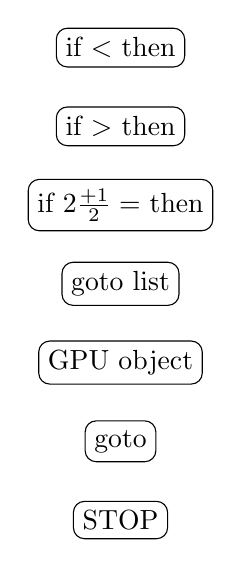
\begin{tikzpicture}
  \node[draw,rounded corners] (ob1) at (0,7) {if $\vde < \vc$ then};
  \node[draw,rounded corners] (ob2) at (0,6) {if $\vdb > \vc$ then};
  \node[draw,rounded corners] (ob3) at (0,5) {if $2 \frac{\vdb+1}{2} = \vc$ then};
  \node[draw,rounded corners] (ob4) at (0,4) {goto \Var{list}};
  \node[draw,rounded corners] (ob5) at (0,3) {GPU object};
  \node[draw,rounded corners] (ob6) at (0,2) {goto };
  \node[draw,rounded corners] (ob7) at (0,1) {STOP};
\end{tikzpicture}
\chapter{The software renderer}

\newcommand{\dy}{\Delta y}
\newcommand{\dx}{\Delta x}

\section{Triangle rendering}

\begin{center}
  \begin{tikzpicture}
    \node (A) at (5,5) {$A$};
    \node (B) at (1,2) {$B$};
    \node (C) at (6,0) {$C$};
    \node (M) at (3,3.5) {};
    \node (N) at (5.3,3.5) {};
    \node (P) at (4.15,3.5) {};
    \draw (A) -- (B) node[pos=0.5,left]{$M$};
    \draw (A) -- (C) node[pos=0.28,right]{$N$};
    \draw (B) -- (C);
    \draw[dashed] (M) -- (N) node[pos=0.5]{$\bullet$} node[pos=0.5,above]{$P$};
    \node (YA) at (0,5) {};
    \node (YM) at (0,3.5) {};
    \node (XM) at (3,-1) {};
    \node (XP) at (4.15,-1) {};
    \draw[dotted] (YA) -- (A);
    \draw[dotted] (YM) -- (M);
    \draw[<->] (YA) -- (YM) node[pos=0.5,left]{$\dy$};
    \draw[dotted] (XM) -- (M);
    \draw[dotted] (XP) -- (P);
    \draw[<->] (XM) -- (XP) node[pos=0.5,above]{$\dx$};
  \end{tikzpicture}
\end{center}

\begin{displaymath}
  \begin{array}{c}
    \begin{array}{c@{\quad\quad\quad}c}
      \left\{
        \begin{aligned}
          x_M & = x_A + \dy \times \frac{x_B - x_A}{y_B - y_A} \\
          v_M & = v_A + \dy \times \frac{v_B - v_A}{y_B - y_A} 
        \end{aligned}
      \right.
      &
      \left\{
        \begin{aligned}
          x_N & = x_A + \dy \times \frac{x_C - x_A}{y_C - y_A} \\
          v_N & = v_A + \dy \times \frac{v_C - v_A}{y_C - y_A} \\
        \end{aligned}
      \right.
    \end{array}
    \\
    \\
    v_P = v_M + \dx \times \frac{v_N - v_M}{x_N - x_M}
  \end{array}
\end{displaymath}

\begin{align*}
v_N - v_M & = \dy \times \left(\frac{v_C - v_A}{y_C - y_A} - \frac{v_B - v_A}{y_B - y_A}\right) \\
& = \dy \times \frac{(v_C - v_A)(y_B - y_A) - (v_B - v_A)(y_C - y_A)}{(y_B - y_A)(y_C - y_A)} \\
\end{align*}

\begin{align*}
x_N - x_M & = \dy \times \left(\frac{x_C - x_A}{y_C - y_A} - \frac{x_B - x_A}{y_B - y_A}\right) \\
& = \dy \times \frac{(x_C - x_A)(y_B - y_A) - (x_B - x_A)(y_C - y_A)}{(y_B - y_A)(y_C - y_A)}
\end{align*}

Thus
\begin{displaymath}
  \frac{v_N - v_M}{x_N - x_M} = \frac{(v_C - v_A)(y_B - y_A) - (v_B - v_A)(y_C - y_A)}{(x_C - x_A)(y_B - y_A) - (x_B - x_A)(y_C - y_A)}
\end{displaymath}

Since this value does not depend on the scanline, this makes a good
reason to handle \emph{only} triangles (this optimisation won't work
on trapezoids for instance).

\smallskip 

Note that
\begin{align*}
(x_C - x_A)(y_B - y_A) - (x_B - x_A)(y_C - y_A) & =
\begin{array}{|cc|} 
  x_C - x_A & x_B - x_A \\
  y_C - y_A & y_B - y_A
\end{array}
\\
& = \det(AC, AB) \\
& = \|AC\| \|AB\| \sin(AC,AB) \\
& = - \|AB\| \|AC\| \sin(AB,AC) \\
& = - \det(AB, AC)
\end{align*}

The triangle is trivial iff this value is null (it represents twice
the area of the triangle). Its sign depends on the orientation of the
triangle.

Thus, one might prefer one of the following expressions:
\begin{align*}
\frac{v_N - v_M}{x_N - x_M} 
& = \frac{(v_C - v_A)(y_B - y_A) - (v_B - v_A)(y_C - y_A)}{(x_C - x_A)(y_B - y_A) - (x_B - x_A)(y_C - y_A)} \\
& = \frac{\begin{array}{|cc|} v_C - v_A & v_B - v_A \\ y_C - y_A & y_B - y_A \end{array}}{\det(AC,AB)} \\
& = \frac{(v_B - v_A)(y_C - y_A) - (v_C - v_A)(y_B - y_A)}{(x_B - x_A)(y_C - y_A) - (x_C - x_A)(y_B - y_A)} \\
& = \frac{\begin{array}{|cc|} v_B - v_A & v_C - v_A \\ y_B - y_A & y_C - y_A \end{array}}{\det(AB,AC)} \\
\end{align*}

\section{Quadrilateral rendering}

\subsection{Trapezoid}

\begin{center}
  \begin{tikzpicture}
    \node (A) at (5,5) {$A$};
    \node (B) at (1,2) {$B$};
    \node (C) at (10,0) {$C$};
    \node (D) at (9,5) {$D$};
    \node (M) at (3,3.5) {};
    \node (N) at (9.3,3.5) {};
    \node (P) at (6.15,3.5) {};
    \draw (A) -- (B) node[pos=0.5,left]{$M$};
    \draw (D) -- (C) node[pos=0.28,right]{$N$};
    \draw (B) -- (C);
    \draw (A) -- (D);
    \draw[dashed] (M) -- (N) node[pos=0.5]{$\bullet$} node[pos=0.5,above]{$P$};
    \node (YA) at (0,5) {};
    \node (YM) at (0,3.5) {};
    \node (XM) at (3,-1) {};
    \node (XP) at (6.15,-1) {};
    \draw[dotted] (YA) -- (A);
    \draw[dotted] (YM) -- (M);
    \draw[<->] (YA) -- (YM) node[pos=0.5,left]{$\dy$};
    \draw[dotted] (XM) -- (M);
    \draw[dotted] (XP) -- (P);
    \draw[<->] (XM) -- (XP) node[pos=0.5,above]{$\dx$};
  \end{tikzpicture}
\end{center}

\begin{displaymath}
  \begin{array}{c}
    \begin{array}{c@{\quad\quad\quad}c}
      \left\{
        \begin{aligned}
          x_M & = x_A + \dy \times \frac{x_B - x_A}{y_B - y_A} \\
          v_M & = v_A + \dy \times \frac{v_B - v_A}{y_B - y_A} 
        \end{aligned}
      \right.
      &
      \left\{
        \begin{aligned}
          x_N & = x_D + \dy \times \frac{x_C - x_D}{y_C - y_D} \\
          v_N & = v_D + \dy \times \frac{v_C - v_D}{y_C - y_D} \\
        \end{aligned}
      \right.
    \end{array}
    \\
    \\
    v_P = v_M + \dx \times \frac{v_N - v_M}{x_N - x_M}
  \end{array}
\end{displaymath}

\begin{align*}
v_N - v_M & = v_D - v_A + \dy \times \left(\frac{v_C - v_D}{y_C - y_D} - \frac{v_B - v_A}{y_B - y_A}\right) \\
& = v_D - v_A + \dy \times \frac{(v_C - v_D)(y_B - y_A) - (v_B - v_A)(y_C - y_D)}{(y_B - y_A)(y_C - y_D)}
\\
x_N - x_M & = x_D - x_A + \dy \times \frac{(x_C - x_D)(y_B - y_A) - (x_B - x_A)(y_C - y_D)}{(y_B - y_A)(y_C - y_D)}
\end{align*}

\begin{align*}
\frac{v_N - v_M}{x_N - x_M} & = ? 
\end{align*}

\subsection{Dividing in triangles}

\begin{center}
  \begin{tikzpicture}
    \node (A) at (5,5) {$A$};
    \node (B) at (1,2) {$B$};
    \node (C) at (10,0) {$C$};
    \node (D) at (9,5) {$D$};
    \node (M) at (3,3.5) {};
    \node (N) at (9.3,3.5) {};
    \node (H) at (6.5,3.5) {};
    \node (P) at (6.15,3.5) {};
    \draw (A) -- (B) node[pos=0.5,left]{$M$};
    \draw (D) -- (C) node[pos=0.28,right]{$N$};
    \draw (B) -- (C);
    \draw (A) -- (D);
    \draw[dotted] (A) -- (C);
    \draw[dashed] (M) -- (N) node[pos=0.5]{$\bullet$} node[pos=0.5,above]{$P$} node[pos=0.56,above]{$H$} node[pos=0.56]{$\times$};
    \node (YA) at (0,5) {};
    \node (YM) at (0,3.5) {};
    \node (XM) at (3,-1) {};
    \node (XP) at (6.15,-1) {};
    \draw[dotted] (YA) -- (A);
    \draw[dotted] (YM) -- (M);
    \draw[<->] (YA) -- (YM) node[pos=0.5,left]{$\dy$};
    \draw[dotted] (XM) -- (M);
    \draw[dotted] (XP) -- (P);
    \draw[<->] (XM) -- (XP) node[pos=0.5,above]{$\dx$};
  \end{tikzpicture}
\end{center}

\begin{align*}
  \frac{v_H - v_M}{x_H - x_M} 
  & = \frac{\begin{array}{|cc|} v_B - v_A & v_C - v_A \\ y_B - y_A & y_C - y_A \end{array}}{\det(AB,AC)} \\
  \frac{v_N - v_H}{x_N - x_H} 
  & = \frac{\begin{array}{|cc|} v_A - v_D & v_C - v_D \\ y_A - y_D & y_C - y_D \end{array}}{\det(DA,DC)} \\
\end{align*}

\end{document}
